\documentclass[12pt]{article}
\usepackage[utf8]{inputenc}
\usepackage[T1]{fontenc}
\usepackage{geometry}
\usepackage{graphicx}
\usepackage{makeidx}
\usepackage{amsmath}
\geometry{margin=2.5cm}

\title{Informe - Práctica \#5}
\author{Tu nombre}
\date{Fecha de entrega}

\begin{document}

	\thispagestyle{empty}
	
	\begin{center}
		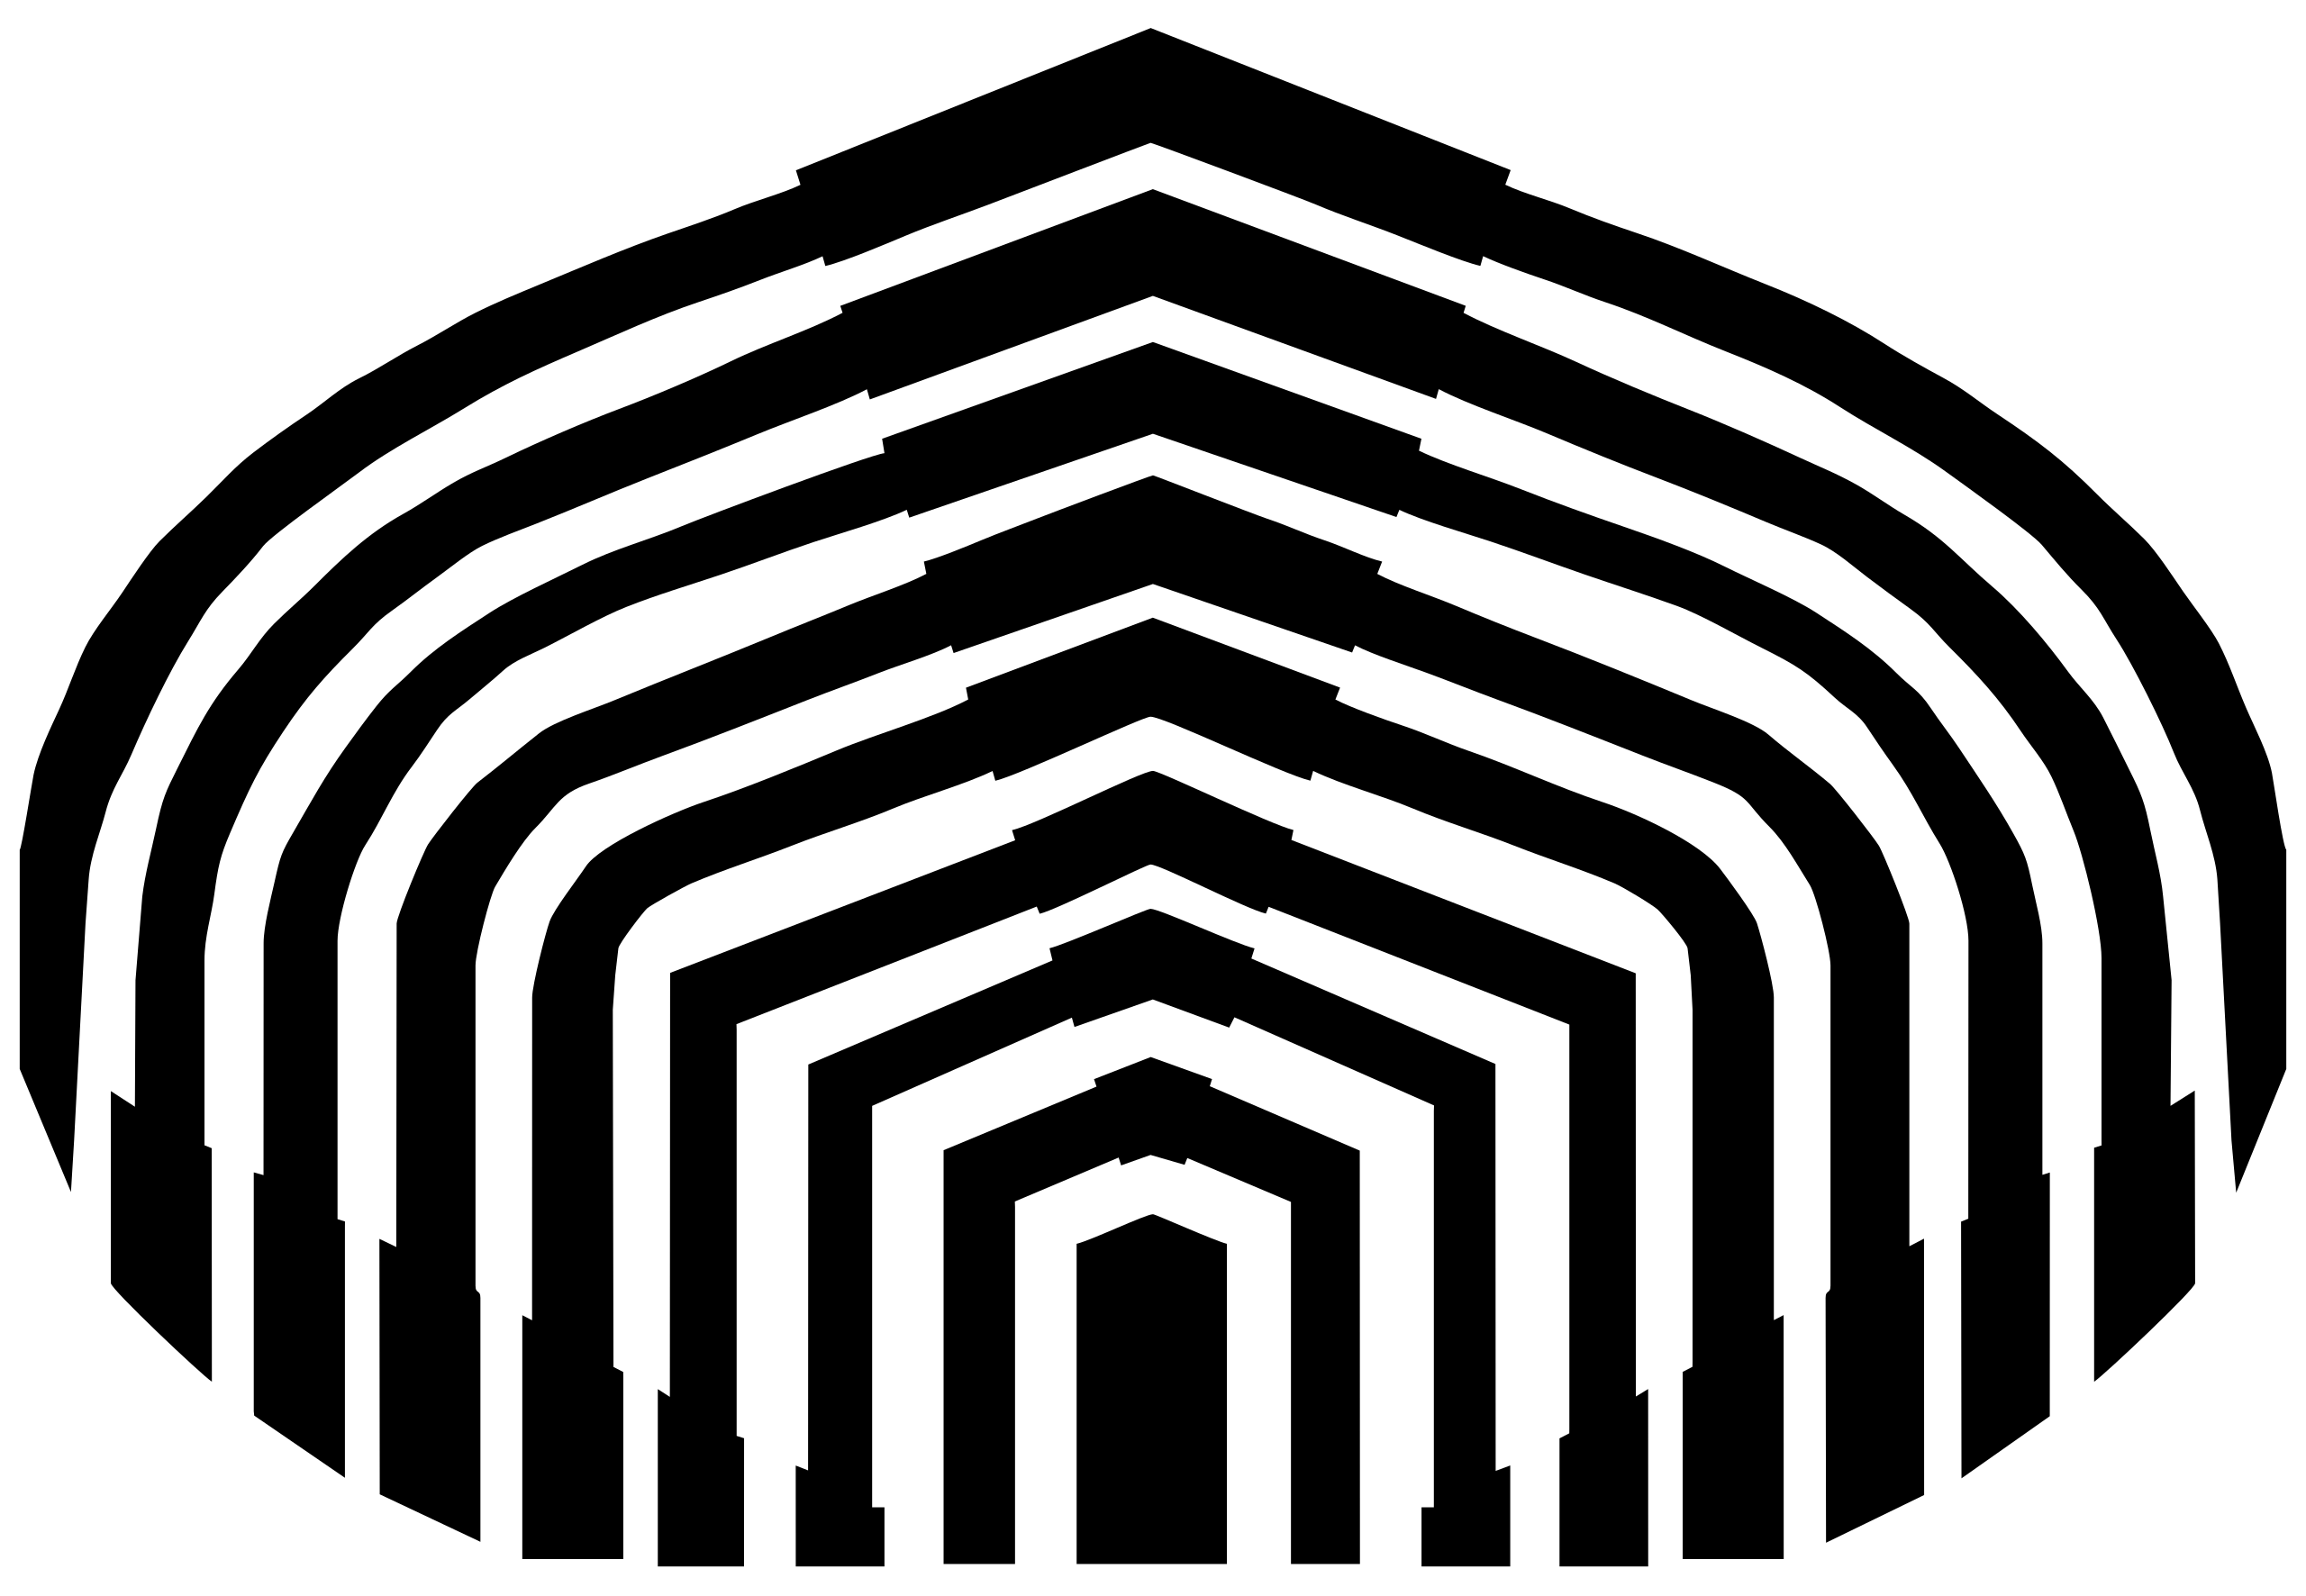
\includegraphics[width=3.1cm,height=2cm]{logo}\\
		UNIVERSIDAD SIMÓN BOLÍVAR\\
		DEPARTAMENTO DE ELECTRÓNICA Y CIRCUITOS\\
		EC1281 - LABORATORIO DE MEDICIONES ELÉCTRICAS\\
		SECCIÓN 1 - GRUPO 1\\
		
		\vspace{7cm}
		\textbf{\Large INFORME - PRÁCTICA \#5}\\
		INTRODUCCIÓN AL LABORATORIO\\
	\end{center}

	\begin{flushleft}
		\vspace{9cm}
		\hfill Integrantes:\\
		\hfill {\large Luis Becerra - 1910557}\\
		\hfill {\large Lorena Rojas - 1910469}\\
	\end{flushleft}

	\newpage
	
	\pagenumbering{roman}
	
	\begin{center}
		\textbf{\large RESUMEN}\\
	\end{center}
	
	\newpage

	\begin{center}
		\textbf{\large ÍNDICE}\\
	\end{center}
	
	\newpage
	\pagenumbering{arabic}
	
	\begin{center}
		\textbf{\large MARCO TEÓRICO}\\
	\end{center}
	
	\newpage
	
	\begin{center}
		\textbf{\large RESULTADOS}\\
	\end{center}

	\section{Trabajo realizado en el laboratorio}
	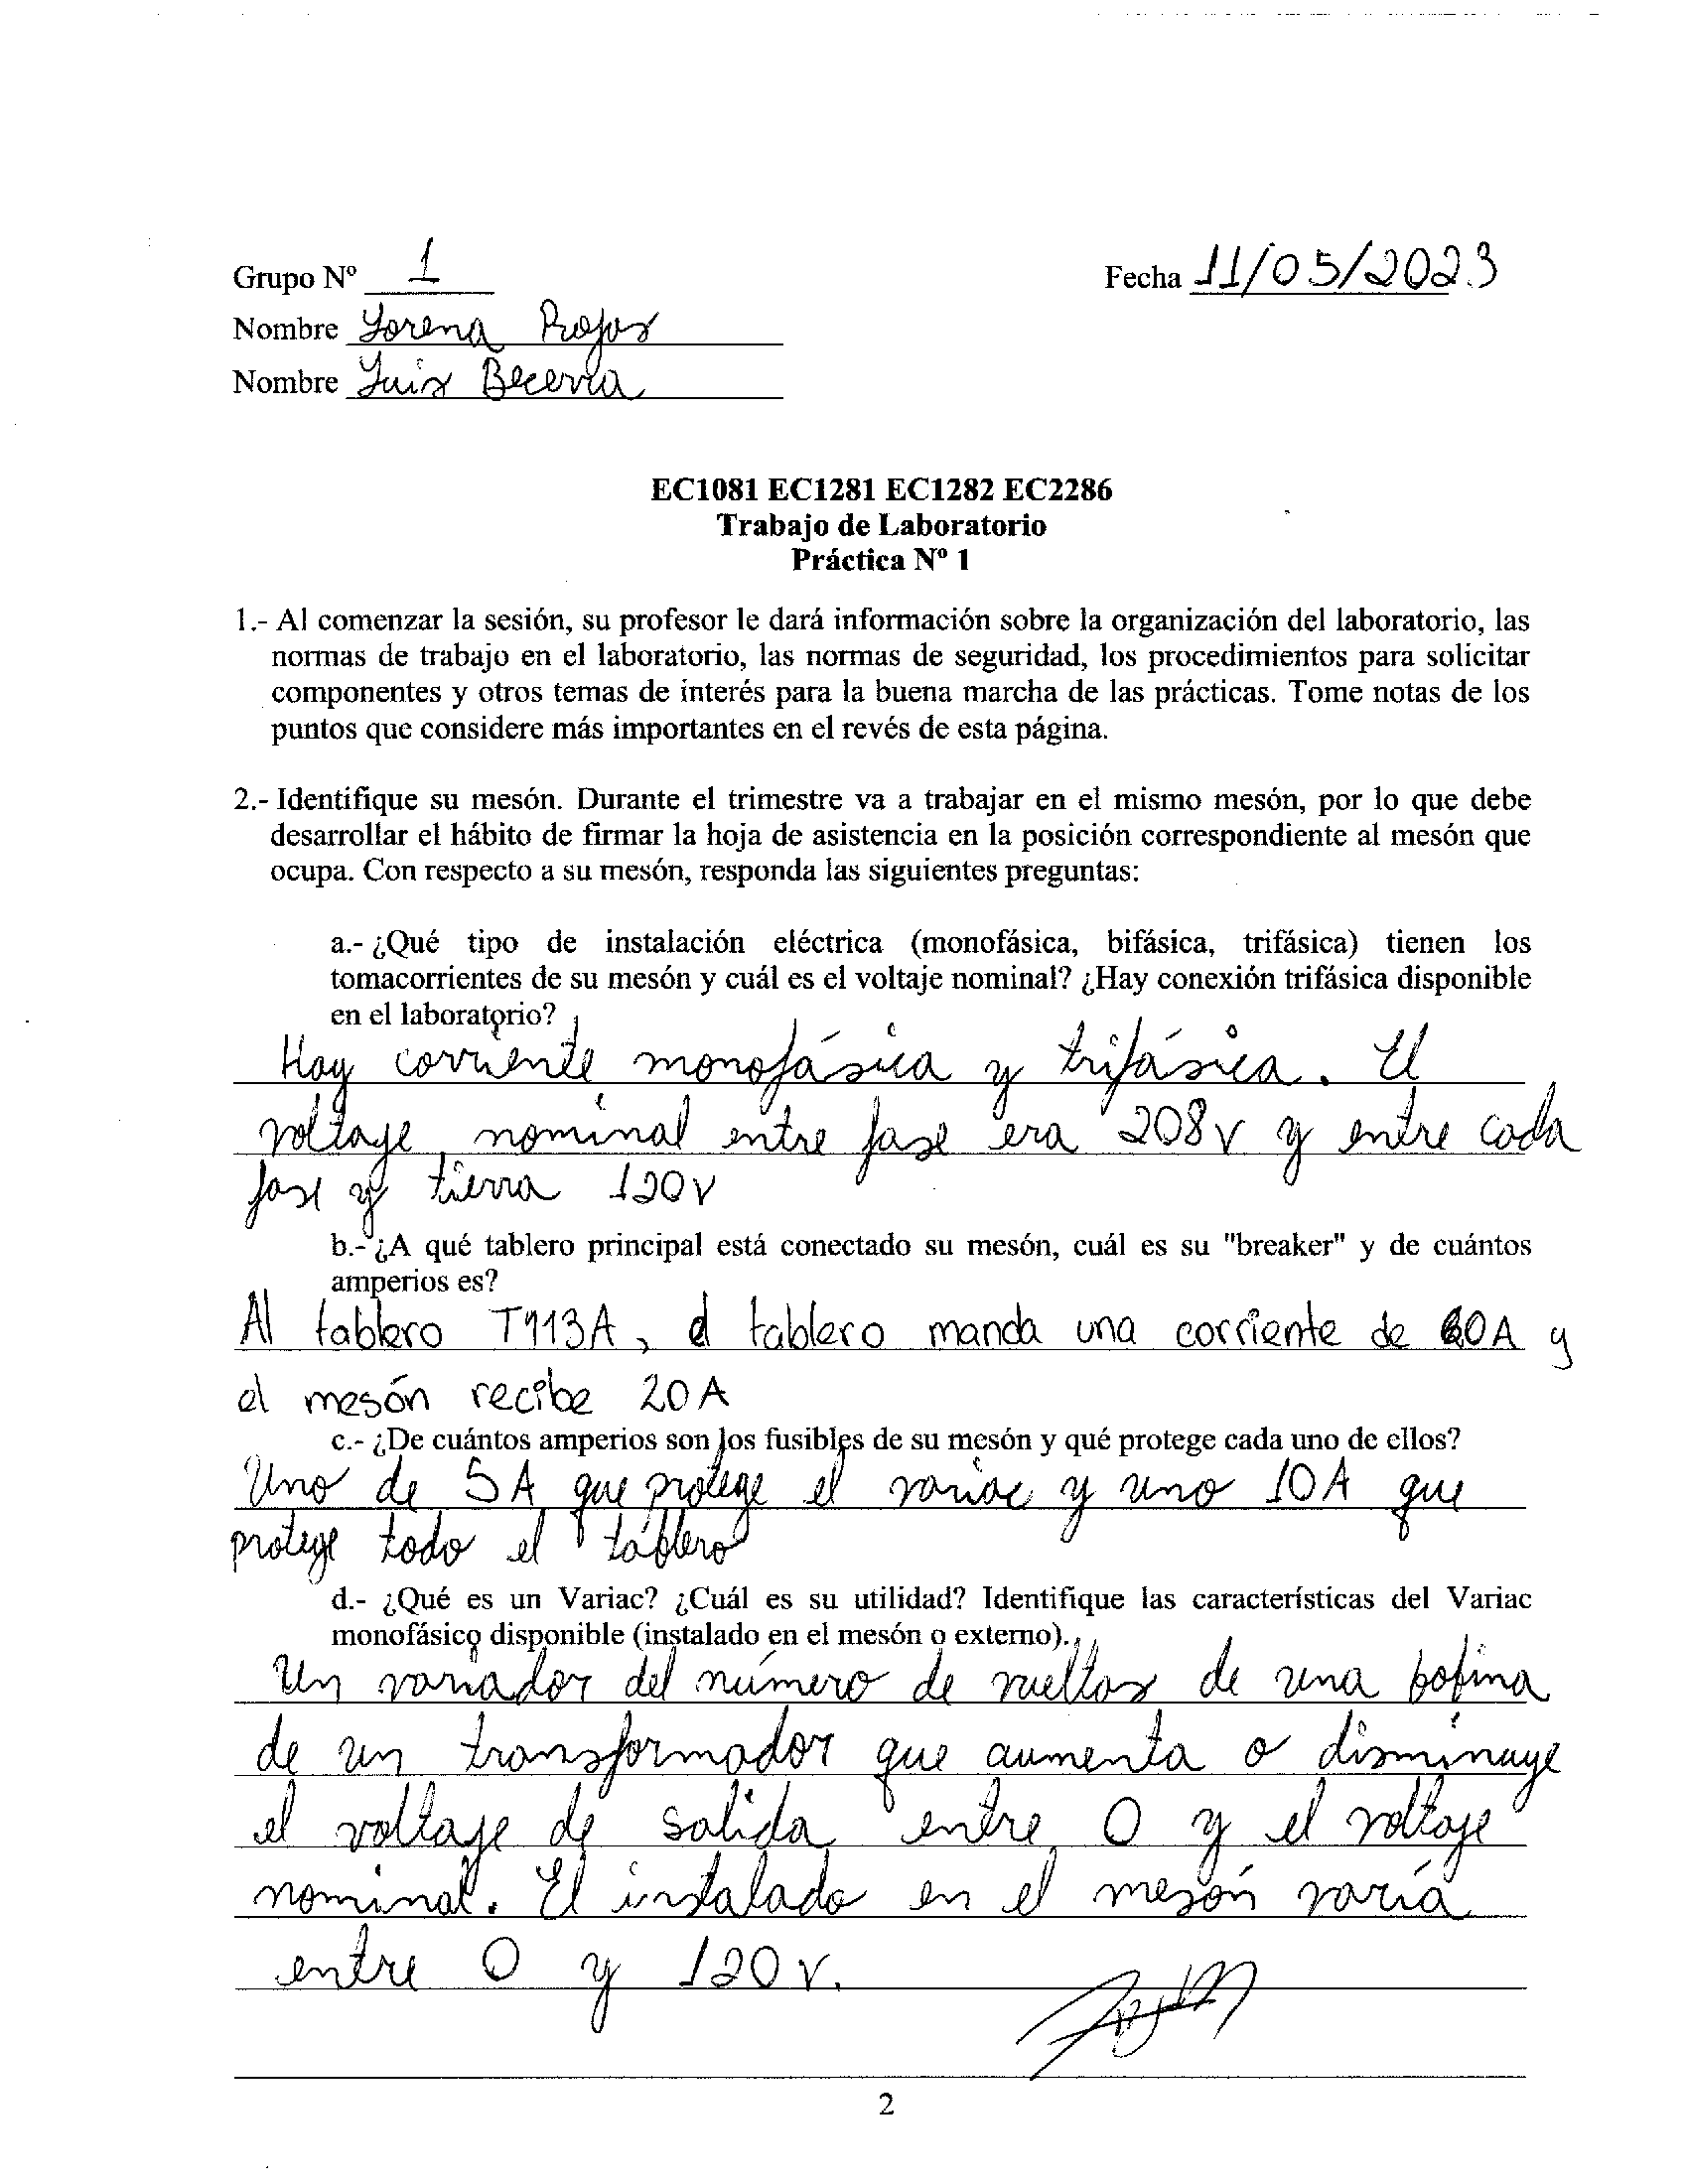
\includegraphics[width=15cm,height=20cm]{anexo1}\\
	
	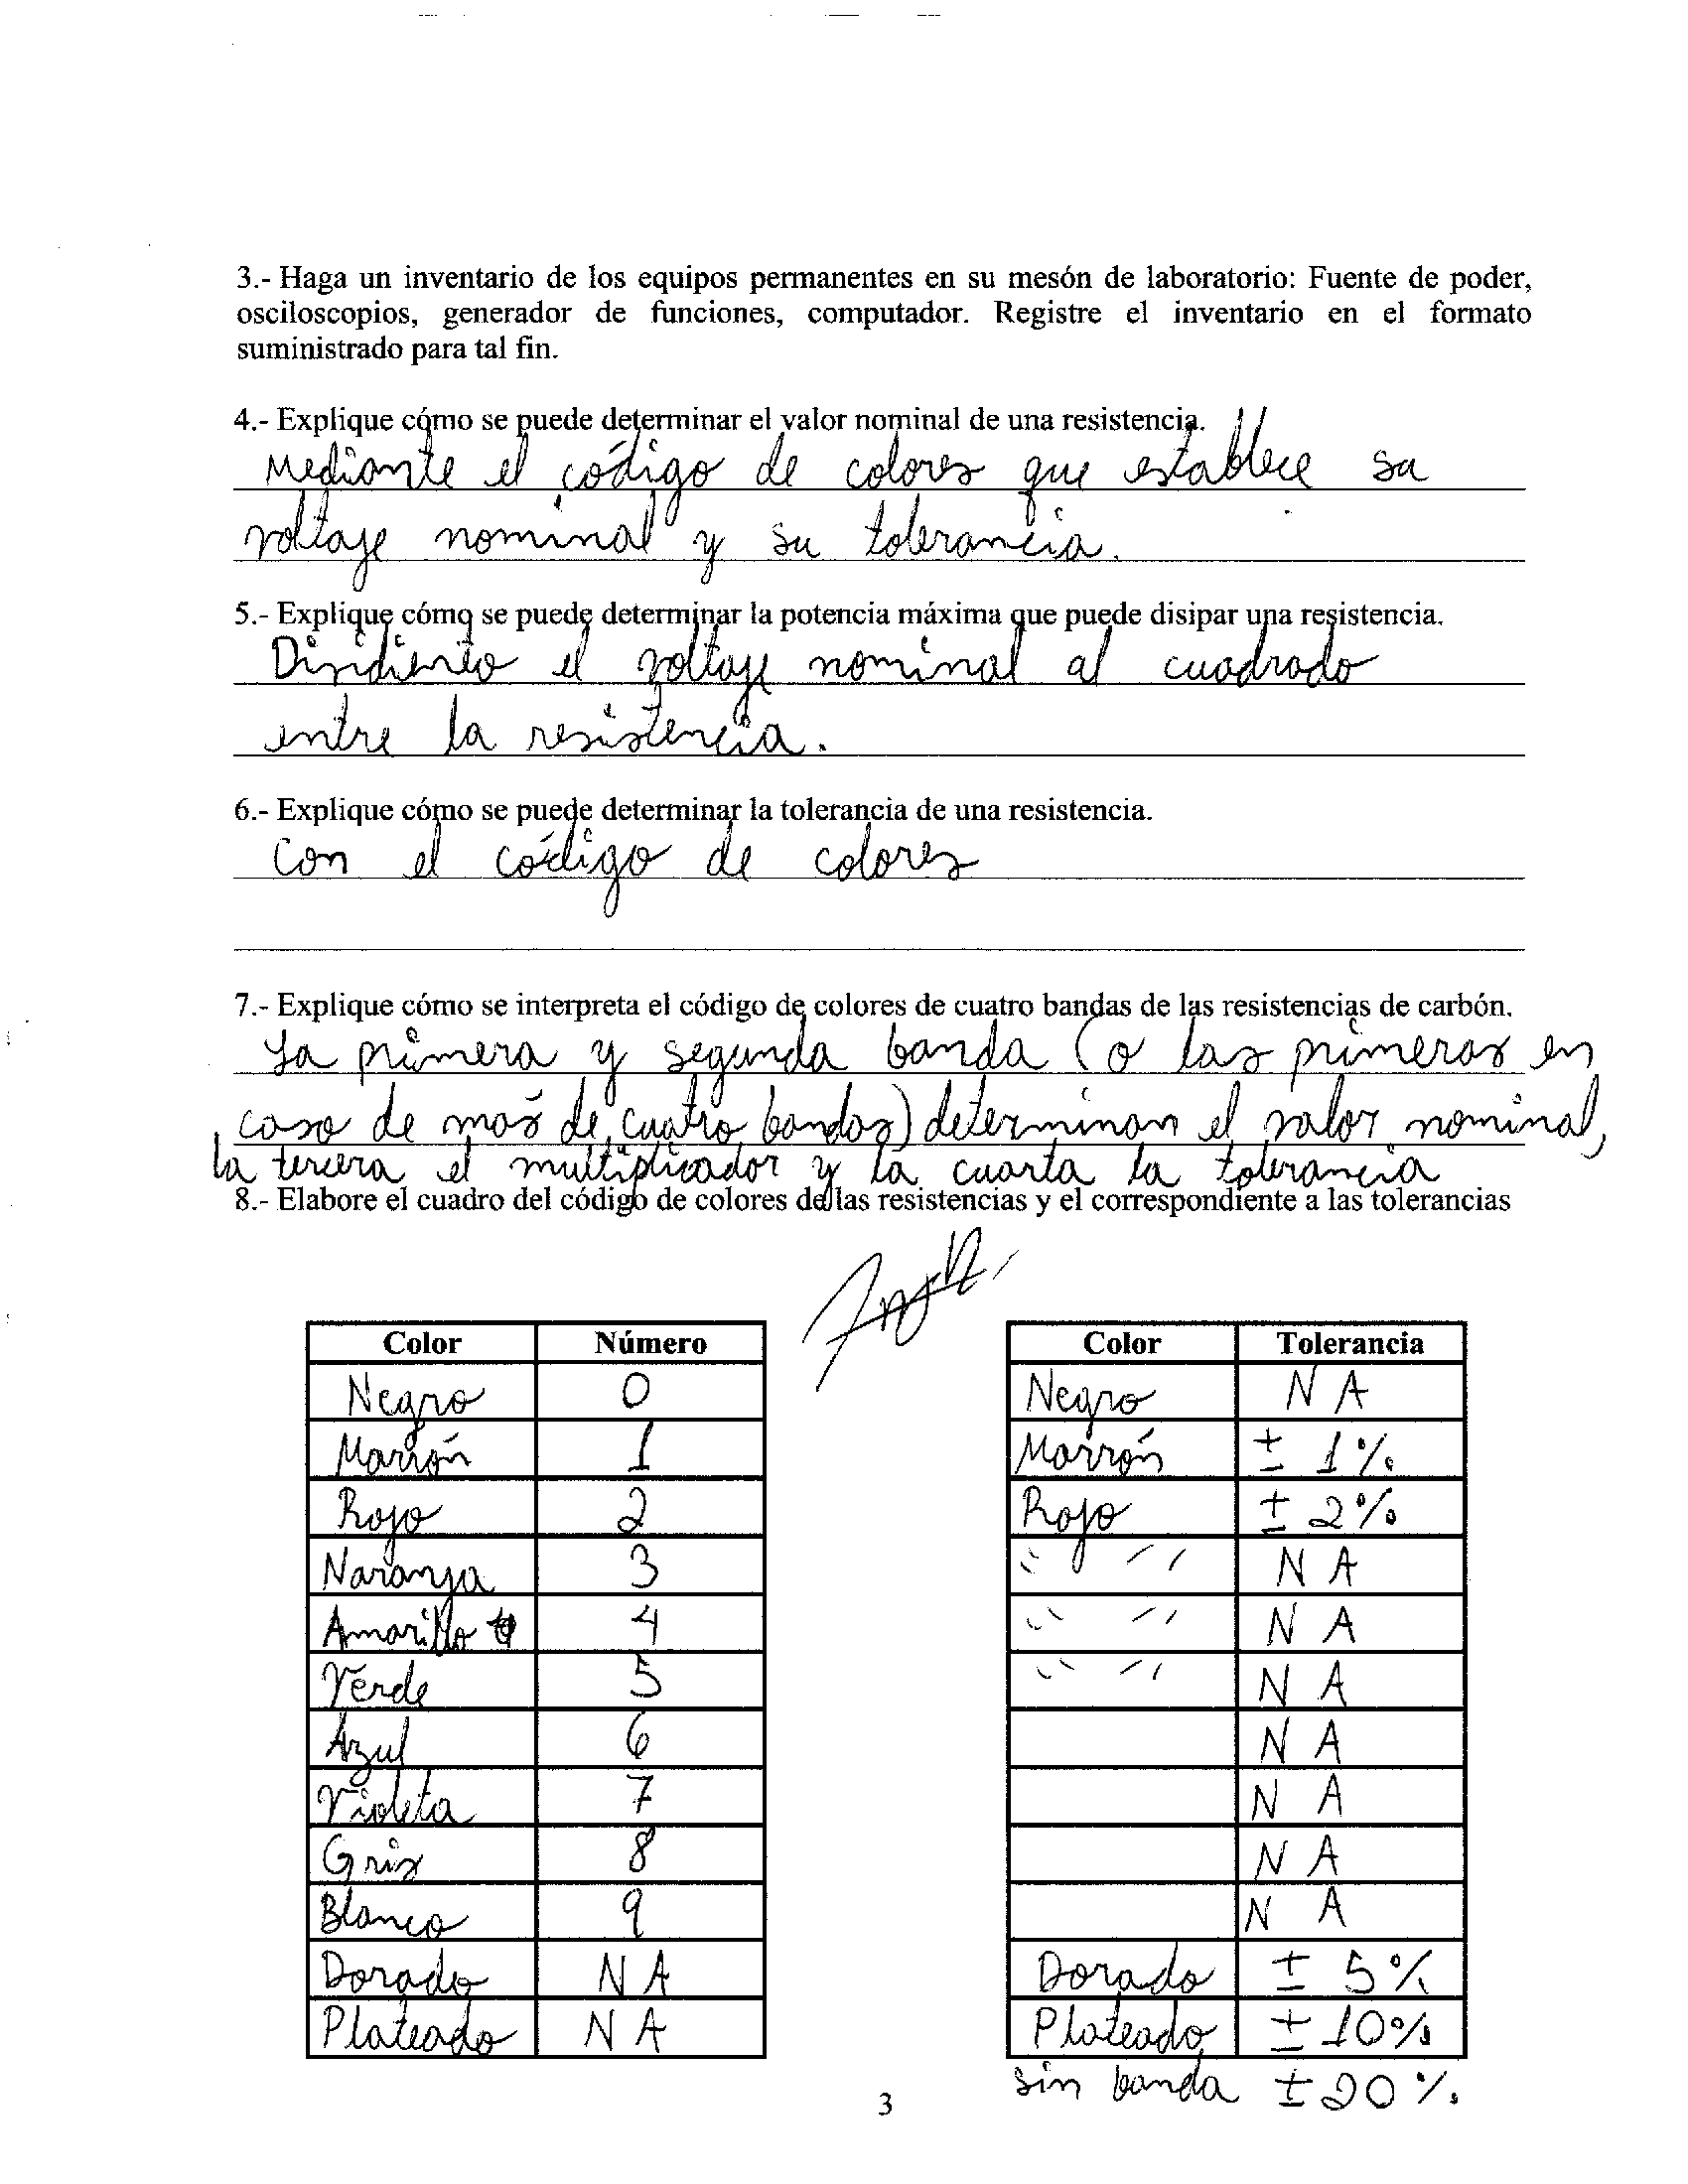
\includegraphics[width=15cm,height=20cm]{anexo2}\\
	
	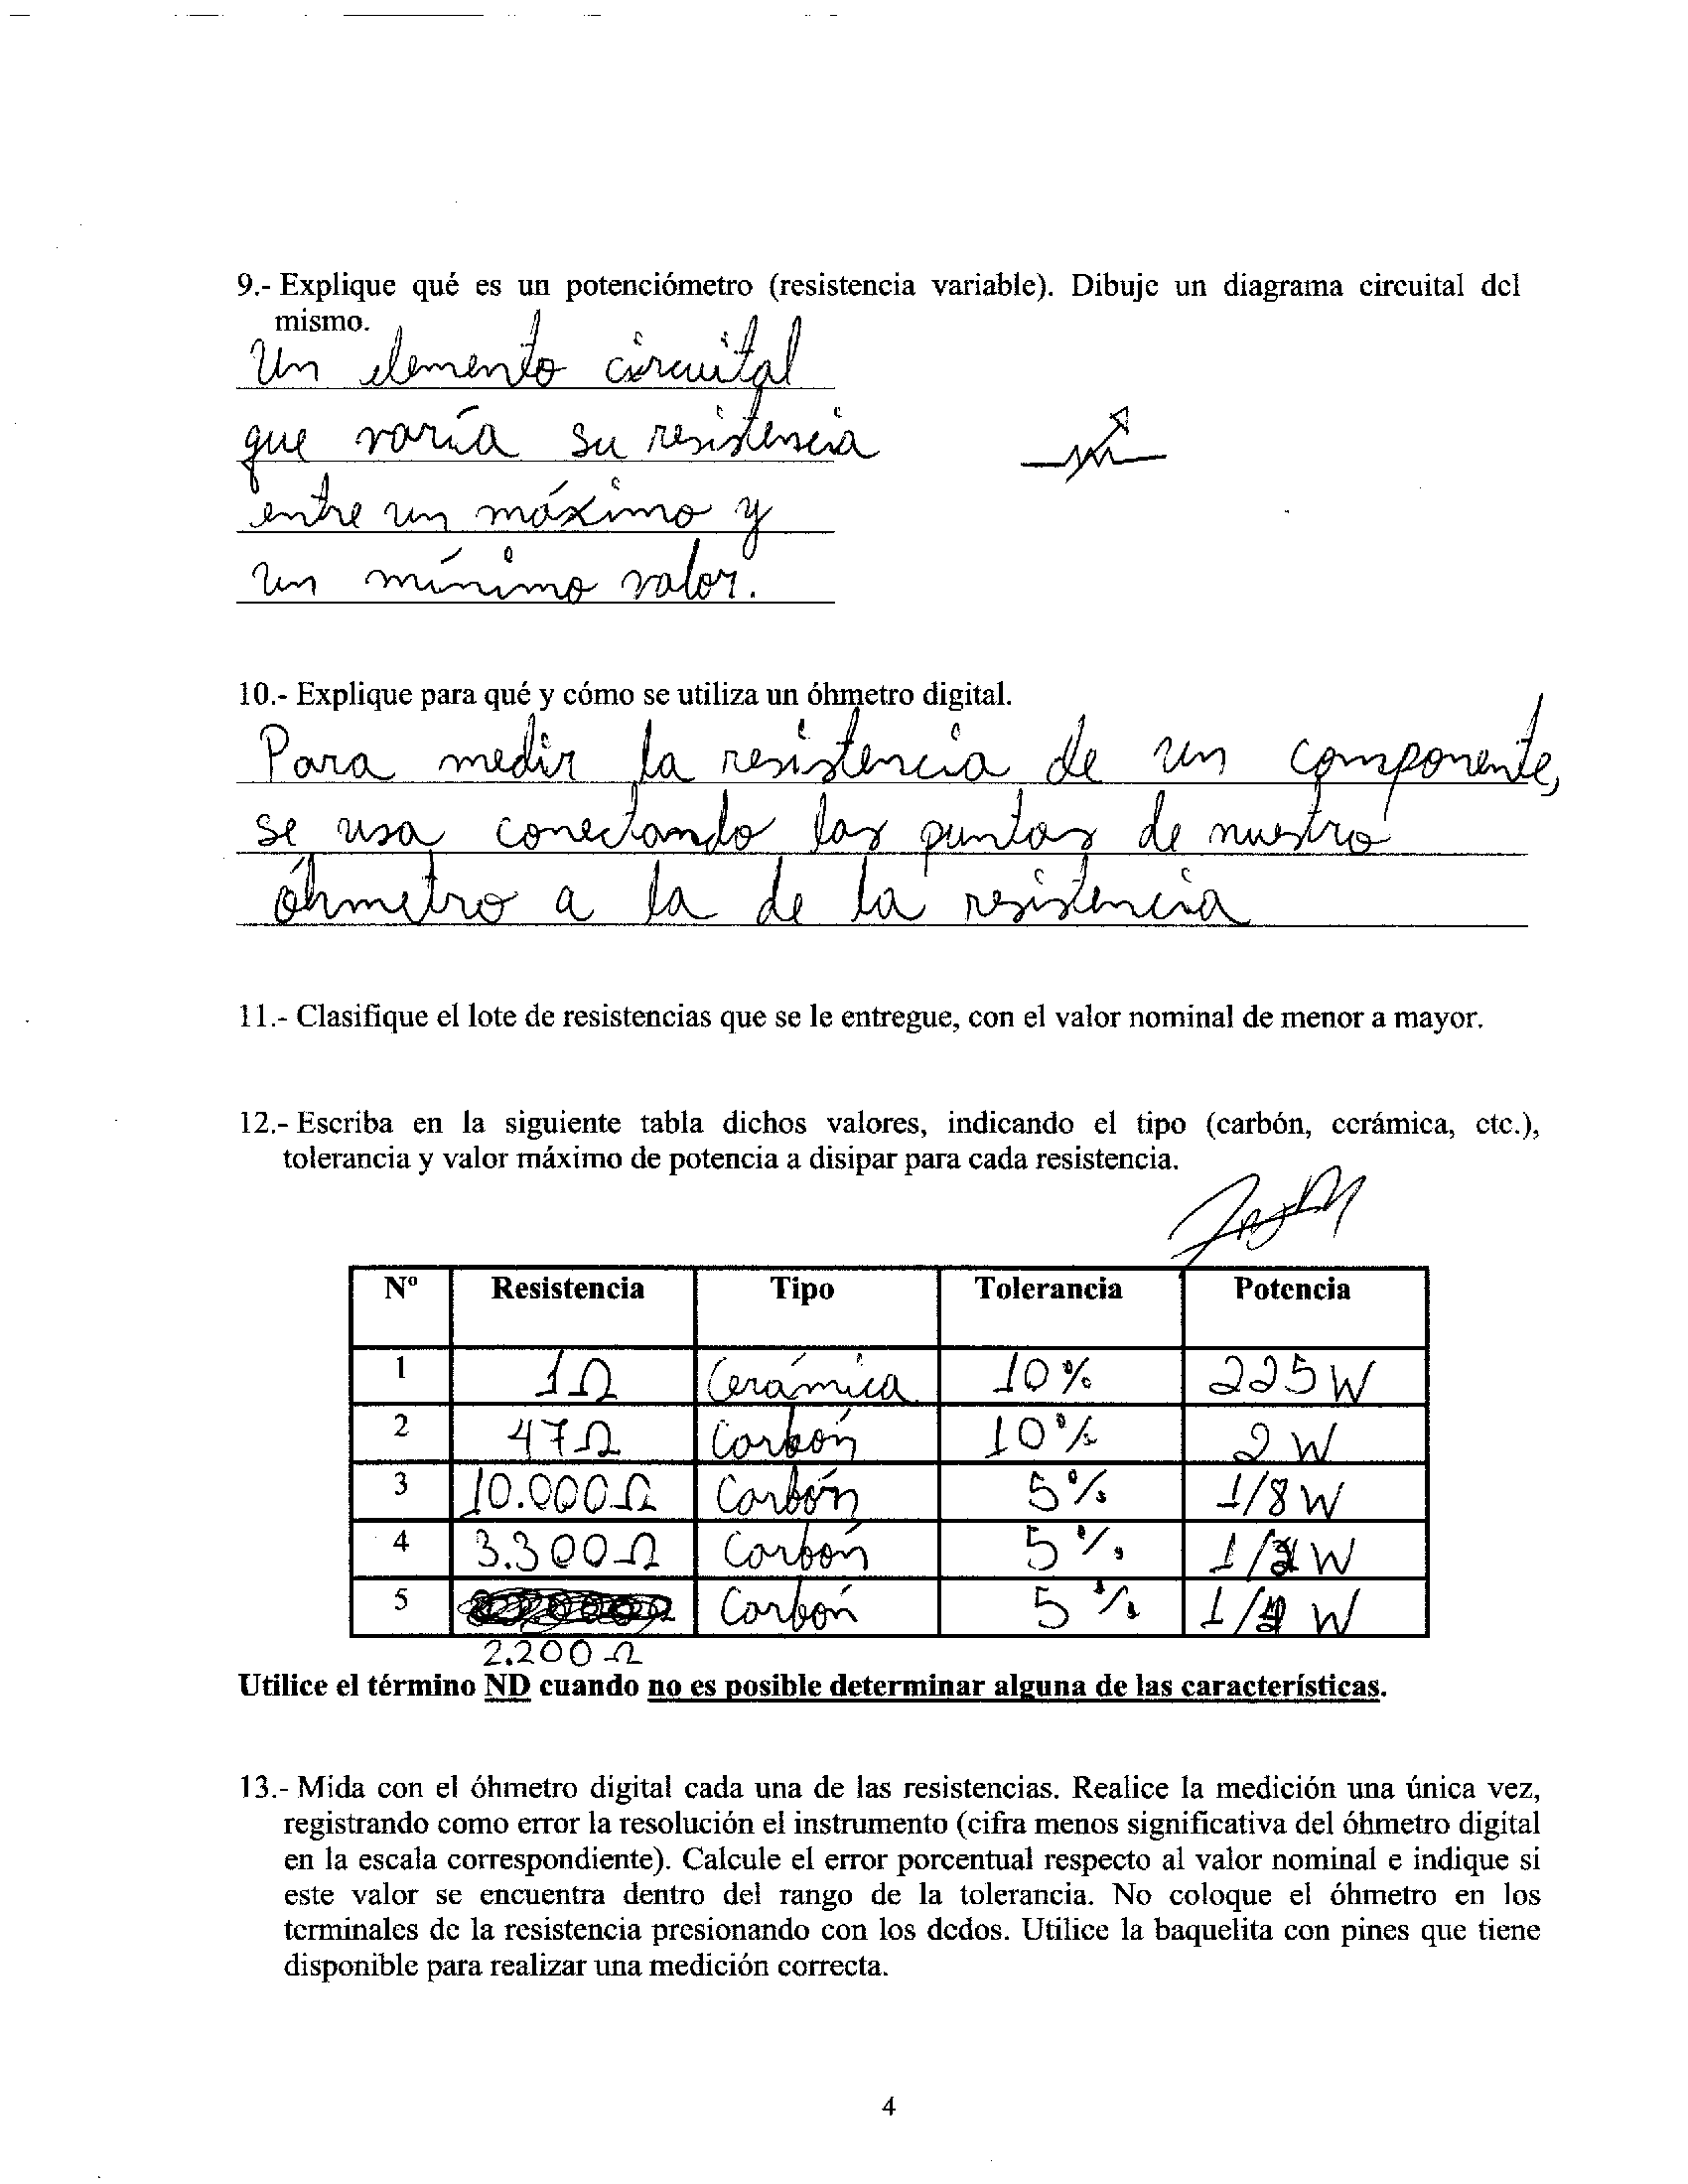
\includegraphics[width=15cm,height=20cm]{anexo3}\\
	
	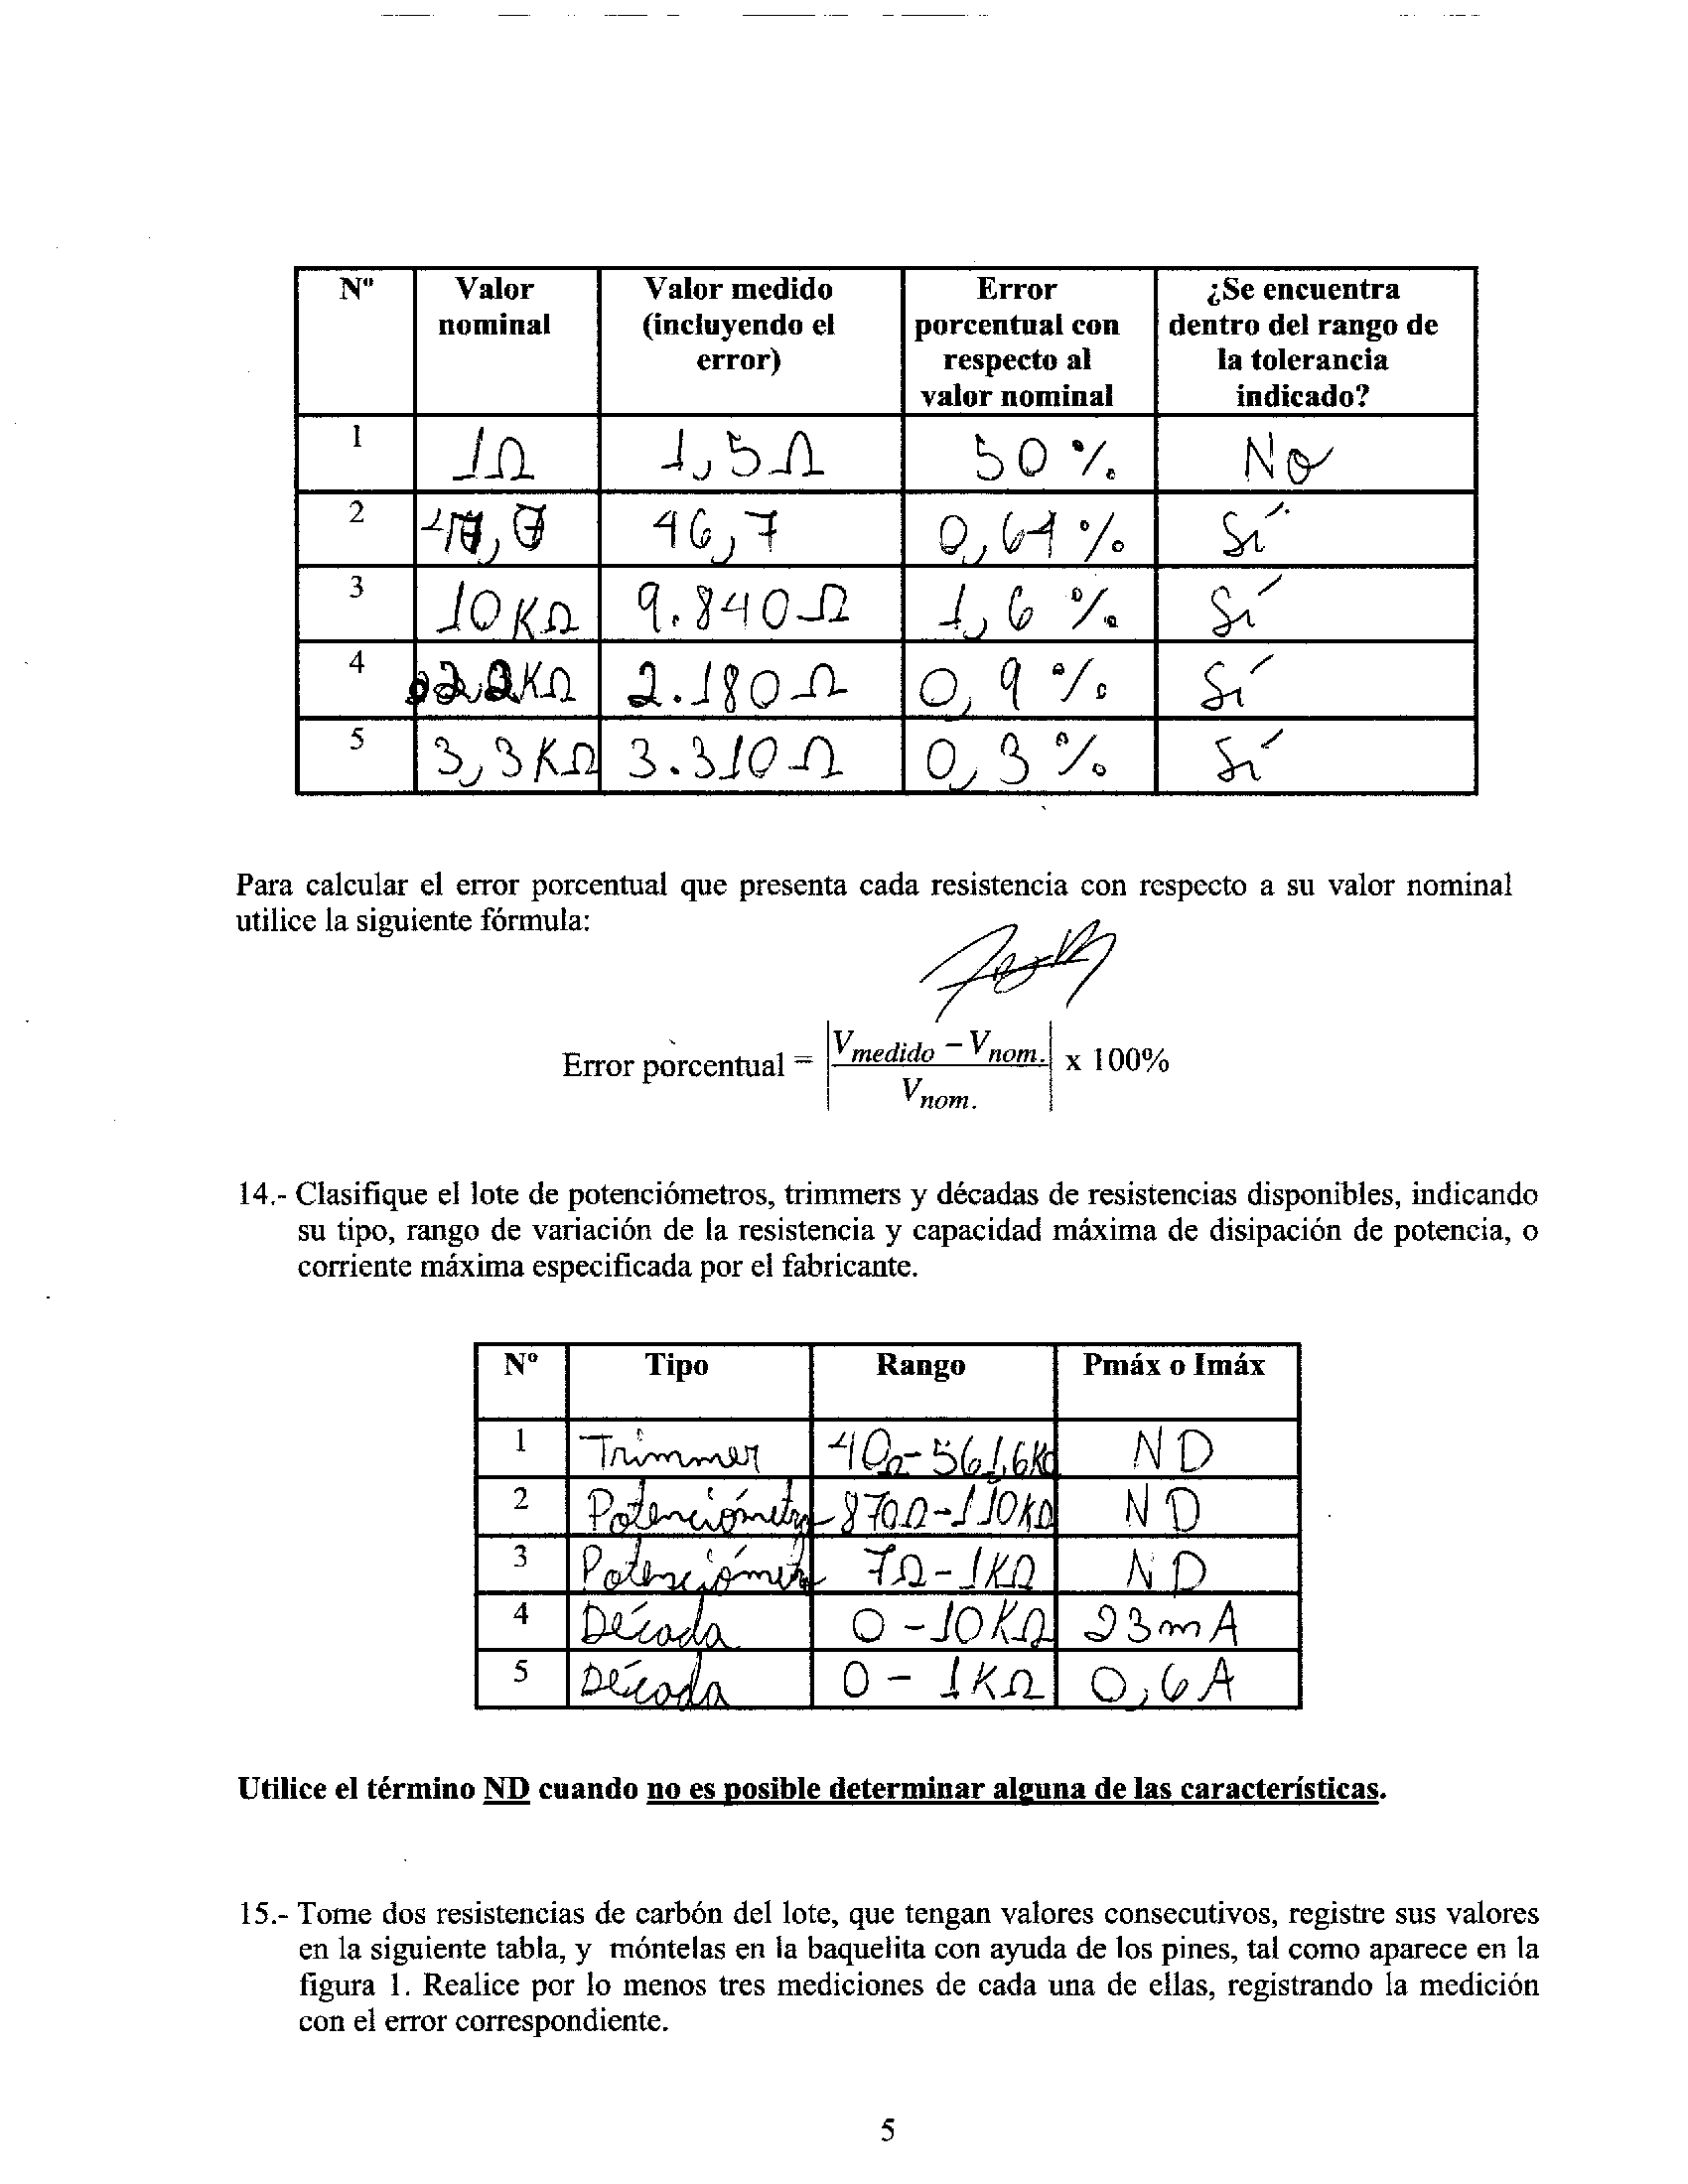
\includegraphics[width=15cm,height=20cm]{anexo4}\\
	
	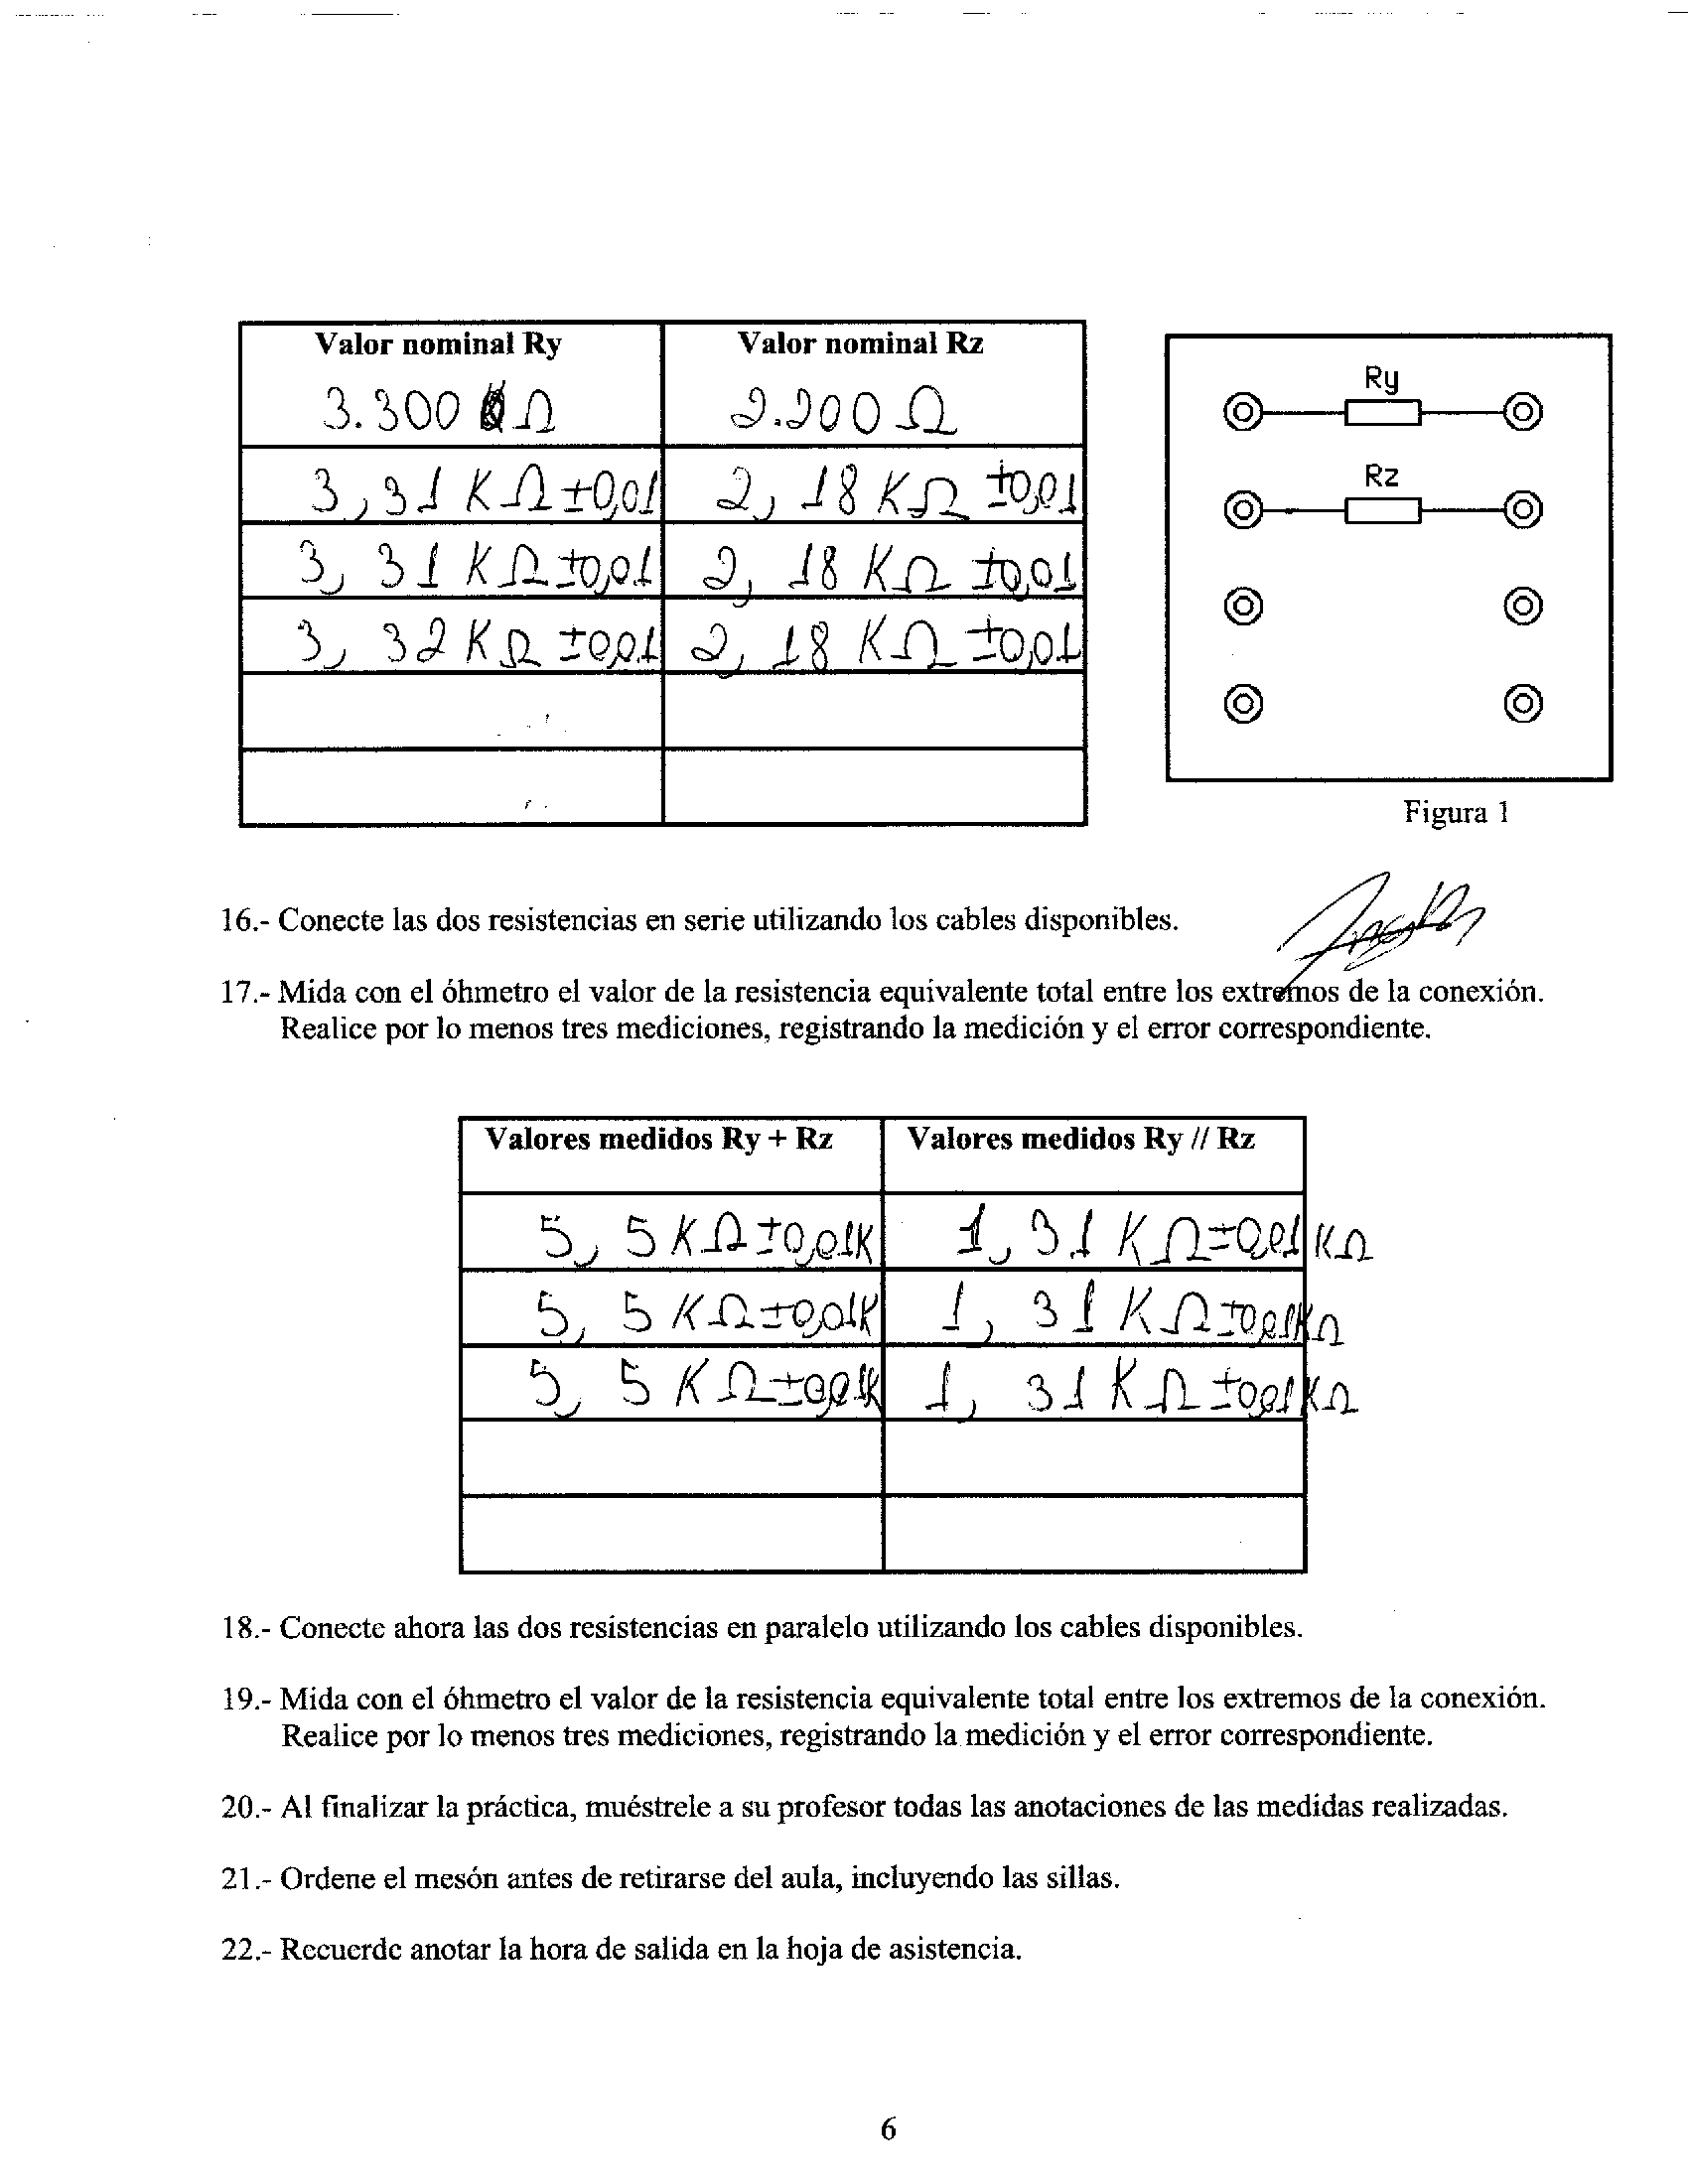
\includegraphics[width=15cm,height=20cm]{anexo5}\\
	
	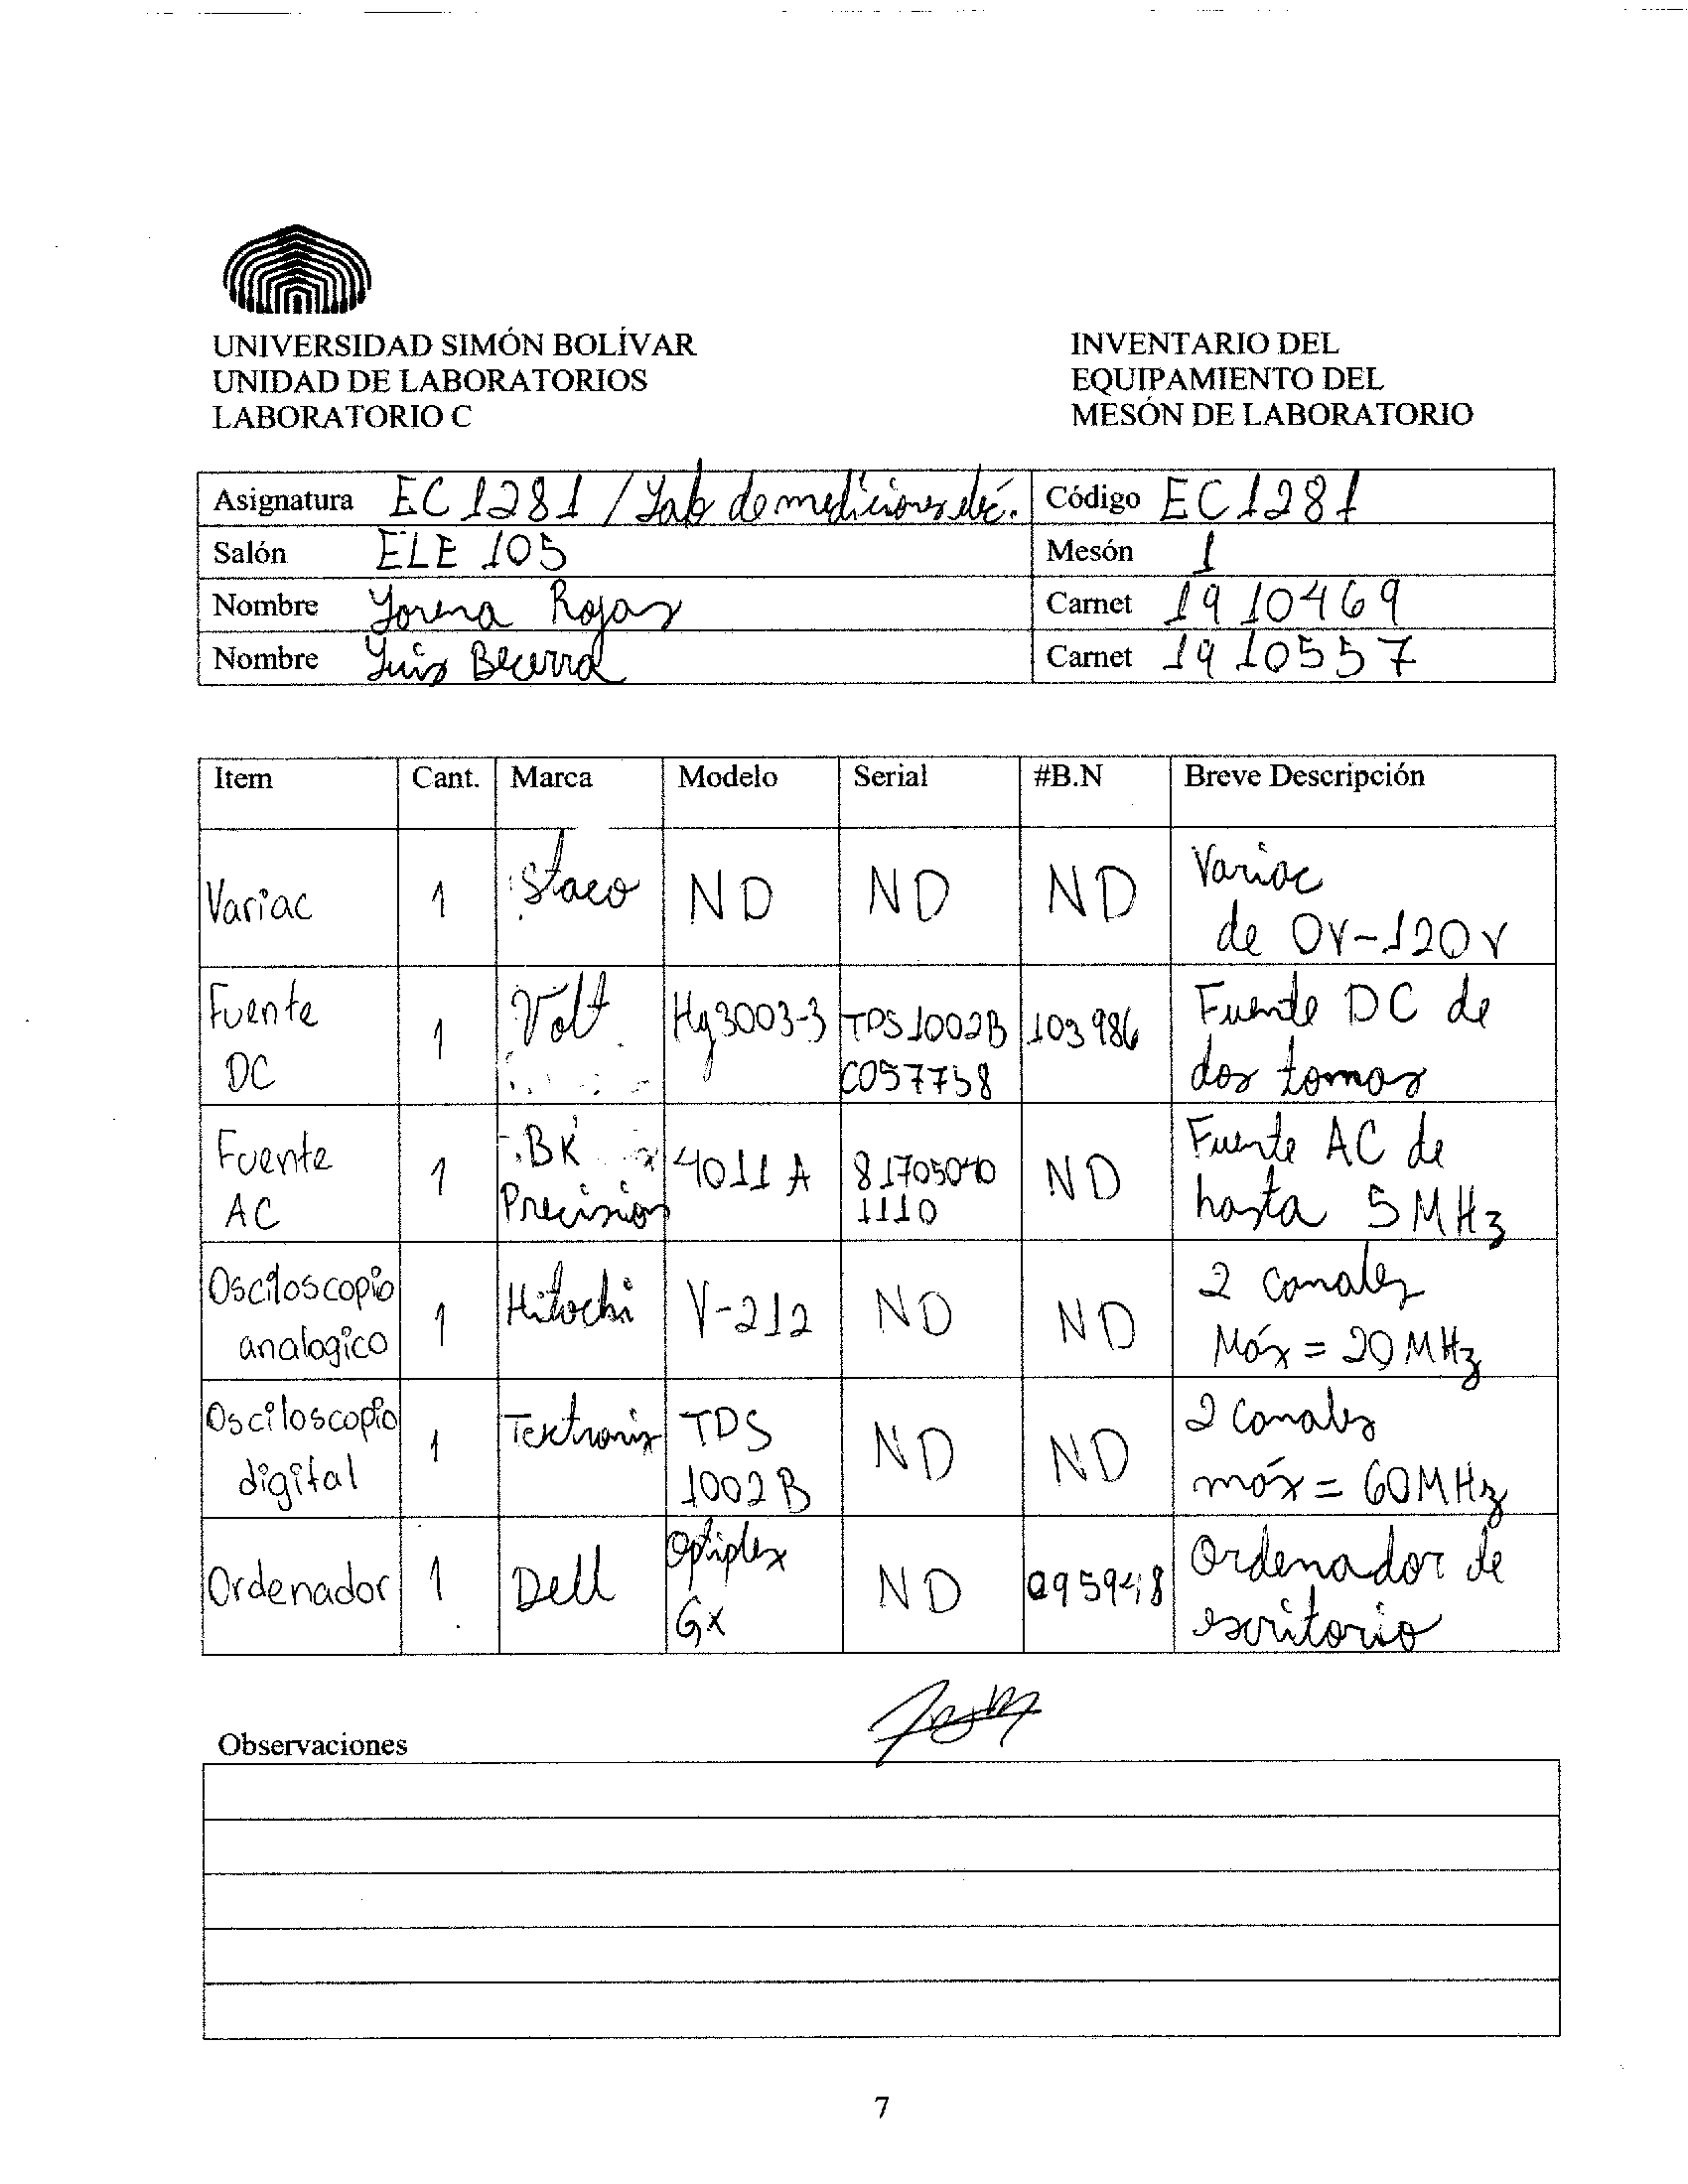
\includegraphics[width=15cm,height=20cm]{anexo6}\\
	
	\newpage
	
	\section{Cálculo de las mediciones}
	
	\subsection{Valor promedio, desviación estándar, error estándar y error total}
	
	\noindent Primero calculamos el valor promedio $<x>$ de nuestras medidas usando la fórmula $<x> = \frac{1}{n}\sum_{i=1}^n x_i$ para $R_y$ y $R_x$.
	\\
	\begin{equation*}
		<R_y> = \frac{3,31 + 3,31 + 3,32}{3} k\Omega = 3,31 k\Omega
	\end{equation*}
	\\
	\begin{equation*}
		<R_x> = \frac{2,18 + 2,18 + 2,18}{3} k\Omega = 2,18 k\Omega
	\end{equation*}
	\\
	\noindent Para el arreglo en serie usamos la fórmula $R_{eq} = \sum_{i=1}^m R_i$ donde $m$ es el número de resistencias en el arreglo y $R_i$ la resistencia i-ésima. Al aplicarlo a nuestras medidas nos queda:\\
	\begin{equation*}
		<R_{xy}> = <R_y> + <R_x> = (3,31 + 2,18)k\Omega = 5,49k\Omega
	\end{equation*}
	\\
	\noindent Al tratar con el arreglo de resistencias en paralelo usamos $R_{eq} = (\sum_{i=1}^m \frac{1}{R_i})^{-1}$ donde $m$ y $R_i$ son análogas a lo que se hizo anteriormente.\\
	\begin{equation*}
		<R_{x||y}> = (\frac{1}{R_y} + \frac{1}{R_x})^{-1} = (\frac{1}{3,31} + \frac{1}{2,18})^{-1}k\Omega = 1,31k\Omega
	\end{equation*}
	\\
	\noindent Luego calculamos la desviación estándar $S_x = \sqrt{\frac{\sum_{i=1}^n(x_i - <x>)^2}{n - 1}}$ para cada resistencia, obteniendo:\\
	\begin{equation*}
		S_y = \sqrt{\frac{(3,31 - 3,31)^2 + (3,31 - 3,31)^2 + (3,32 - 3,31)^2}{3 - 1}} = 5 \times 10^{-5} k\Omega
	\end{equation*}
	\\
	\begin{equation*}
		S_x = \sqrt{\frac{(2,18 - 2,18)^2 + (2,18 - 2,18)^2 + (2,18 - 2,18)^2}{3 - 1}} = 0 k\Omega
	\end{equation*}
	\\
	\noindent La calculamos también para las medidas de los arreglos en serie y paralelo:\\
	\begin{equation*}
		S_{xy} = \sqrt{\frac{(5,5 - 5,5)^2 + (5,5 - 5,5)^2 + (5,5 - 5,5)^2}{3 - 1}} = 0 k\Omega
	\end{equation*}
	\\
	\begin{equation*}
		S_{x||y} = \sqrt{\frac{(1,31 - 1,31)^2 + (1,31 - 1,31)^2 + (1,31 - 1,31)^2}{3 - 1}} = 0 k\Omega
	\end{equation*}
	\\
	\noindent Tendremos que para calcular el error total usaremos $\Delta Z = \sqrt{\sigma_{est}^2 + \sigma_{nom}^2}$, donde $\sigma_{est} = \frac{S_x}{\sqrt n}$ y $\sigma_{nom}$ es el error nominal determinado por el instrumento. Acá tendremos que el error nominal es equivalente al error de apreciación ya que el proceso no resultó en ningún error de definición, exactitud ni interacción.\\
	\begin{equation*}
	 	\Delta Z_x = \sqrt{(\frac{S_x}{\sqrt n})^2 + \sigma_{nom}^2} = \sqrt{(\frac{0}{\sqrt 3})^2 + 0,01^2} = 0,01k\Omega
	\end{equation*}
	 \\
	 \begin{equation*}
	 	\Delta Z_y = \sqrt{(\frac{S_y}{\sqrt n})^2 + \sigma_{nom}^2} = \sqrt{(\frac{5\times 10^{-5}}{\sqrt 3})^2 + 0,01^2} = 0,01k\Omega
	 \end{equation*}
	 \\
	 \begin{equation*}
	 	\Delta Z_{xy} = \sqrt{(\frac{S_{xy}}{\sqrt n})^2 + \sigma_{nom}^2} = \sqrt{(\frac{0}{\sqrt 3})^2 + 0,01^2} = 0,01k\Omega
	 \end{equation*}
	 \\
	 \begin{equation*}
	 	\Delta Z_{x||y} = \sqrt{(\frac{S_{xy}}{\sqrt n})^2 + \sigma_{nom}^2} = \sqrt{(\frac{0}{\sqrt 3})^2 + 0,01^2} = 0,01k\Omega
	 \end{equation*}
	 \\
	 \subsection{Propagación de errores}
	 \noindent Si bien realizamos medidas de las resistencias en serie y paralelo, es conocido que también podemos llegar a tales valores mediante operaciones con resistencias, como se hizo en páginas anteriores, a dichas medidas es necesario aplicarles la propagación de errores.
	 \\
	 
	 \noindent Tendremos que para nuestras resistencias en serie $\Delta R_{eq} = \Delta R_x + \Delta R_y$, quedando:\\
	 \begin{equation}
	 	\Delta R_{xy} = 0,01 + 0,01 = 0,02k\Omega
	 \end{equation}
 	 \\
 	 
 	 \noindent Obteniendo que $R_x + R_y = 5,49k\Omega \pm 0,02k\Omega$.\\
 	 
 	 \noindent Para las resistencias en paralelo tendremos que $\Delta R_{x||y} = \frac{<R_y>^2}{(<R_x> + <R_y>)^2}\Delta R_x + \frac{<R_x>^2}{(<R_x> + <R_y>)^2}\Delta R_y$ que al desarrollar nos queda:\\
 	 
 	 \begin{equation}
 	 	\Delta R_{x||y} = \frac{3,31^2}{(2,18 + 3,31)^2}0,01 + \frac{2,18^2}{(2,18 + 3,31)^2}0,01 = 0,005k\Omega
 	 \end{equation}
 	 \\
 	 
 	 \noindent Quedando que $R_{x||y} = 1,31k\Omega \pm 0,005k\Omega$
 	 
 	 \newpage
 	 
 	 \begin{center}
 	 	\textbf{\large ANÁLISIS DE RESULTADOS}\\
 	 \end{center}
 	 
 	 \section*{Error estándar del promedio vs error nominal}
 	 
 	 \noindent A efectos de estas mediciones, se puede evidenciar que el error estandar del promedio es mínimo cuando no es cero, por lo cual la única limitante se podría decir que es la calidad de la medida de nuestra herramienta, en otras palabras, aumentar el número de medidas no representaría una mejora substancial con respecto a los resultados obtenidos con tan sólo tres medidas. \\
 	 
 	 \section*{Resultado final vs mediciones directas de los arreglos en serie y paralelo}
 	 
 	 \noindent Ambas mediciones dieron un resultado sumamente preciso, sin embargo, cabe a destacar que la medida directa fue la más precisa en el caso del circuito en serie ya que arroja la medición con un margen de error más pequeño , mientras que en el arreglo paralelo, fue la medición indirecta la que resultó en un menor error, esto se debe a que en serie,  al medir las dos resistencias, el error propagado va directamente relacionado con la suma de los dos errores medidos, mientras que en paralelo, los errores medidos se disminuyen al realizar las operaciones algebraicas.\\
 	 
 	 \section*{Rango de tolerancia de las resistencias}
 	 
 	 \noindent Las medidas tomadas revelan que los valores obtenidos sí están dentro del rango de tolerancia, luego, al proyectar eso hacia el arreglo en serie o en paralelo se encuentra con que efectivamente esta proporción se mantiene.\\
 	 
 	 \newpage
 	 
 	 \begin{center}
 	 	\textbf{\large CONCLUSIONES}\\
 	 \end{center}
  
	  \noindent Como se pudo observar, el manejo de los errores es un aspecto fundamental cuando se realiza un arreglo eléctrico de cualquier tipo, durante ese proceso, aunque se tengan herramientas de calidad, igualmente es indispensable ser rigurosos con las mediciones y seguir protocolos tanto por seguridad como para evitar que las medidas se vean perjudicadas por cualquier factor humano. Mientras más cautela se tenga, más se reducirá el margen de error y en consecuencia se tendrán medidas de mejor calidad.\\
	  
	  \noindent También cabe destacar que es excelente idea siempre que sea posible, probar con medidas directas e indirectas, ya que como se pudo evidenciar, en ocasiones una o la otra tendrá mayor precisión y si se tiene la oportunidad de probarlo, no sería una idea desacertada.\\
	  
	  \noindent En la medida en que se vaya avanzando, es necesario siempre tener presente que los errores son parte natural de un proceso de investigación y que si bien no se pueden erradicar, se pueden disminuir al mínimo si se siguen prácticas adecuadas al llevar a cabo cualquier tipo de experimento con arreglos eléctricos.
	  
	  \newpage
	  
	  \begin{center}
	  	\textbf{\large COMENTARIOS FINALES}\\
	  \end{center}
  	  
  	  \noindent Esta es la primera aproximación práctica a la carrera que se tiene en ingeniería electrónica, una práctica que recuerda al rigor metodológico que se promueve durante el laboratorio de física 1 a la hora de trabajar con mediciones y presenta un abre boca de cómo se da el tratamiento de mediciones cuando se trata de fenómenos eléctricos.\\
  	  
  	  \noindent Se conocieron algunos componentes eléctricos básicos, las herramientas del laboratorio y se dió un vistazo a el procedimiento que se seguirá durante el curso para trabajar en el laboratorio, una experiencia enriquecedora y sumamente interesante.
  	  
\end{document}